\section{History of DNA and genes}

In the winter of 1868/9, Swiss physician and biologist, Johannes Friedrich Miescher isolated an unknown substance from the nuclei of cells\cite{dahm2008discovering}. This substance was unlike anything he had observed before; it was resistant to protease, lacked sulphur, and contained a large amount of phosphorous. He recognised that he had isolated a novel substance and as it was from the nucleus, he named it nuclein. In 1881, Albrecht Kossel determined that nuclein was composed of five bases: adenine (A), cytosine (C), guanine (G), thymine (T), and uracil (U). Later in 1889, Richard Altmann discovered that nuclein was acidic (due to presence of phosphorous) and renamed nuclein as nucleic acid. The basic component of deoxyribonucleic acid (DNA) was deduced by Phoebus Levene in 1909, where he discovered that DNA consisted of an acid, an organic base, and a sugar; he also showed that these components were linked together as phosphate-sugar-base to form units, which he termed nucleotides. This sugar-phosphate backbone forms the structural framework of nucleic acids and makes DNA highly stable. In 1928, Frederick Griffith demonstrated that heritable traits could be transferred between dead and live bacteria and that provided the first clue that a ``transforming factor" existed\cite{griffith1928significance}. It wasn't until 1944, when Oswald Avery, Colin MacLeod, and Maclyn McCarty demonstrated that deoxyribonucleodepolymerase (an enzyme that degrades DNA) destroyed the ``transforming factor", that it was hypothesised DNA was the genetic material\cite{avery1944studies}. This was later confirmed in 1952 by Alfred Hershey and Martha Chase, by demonstrating that when bacteriophages infected bacteria, only their DNA would enter into the cytoplasm of the bacteria, while their protein remained outside\cite{hershey1952independent}.

While Phoebus Levene proposed that DNA was made up equal amounts of A, C, G, and T, it was later discovered by Erwin Chargaff that DNA should have a 1:1 ratio of pyrimidine (C, T, and U) and purine (A and G) bases\cite{pmid14938364, pmid14945441}; this became known as Chargaff's rules. The three-dimensional (3D) structure of DNA was solved by Francis Crick and James Watson in 1953\cite{WATSON_1953} after gaining insight from an X-ray diffraction image taken by Rosalind Franklin and from Chargaff's rules. The 3D structure of DNA showed how adenines paired with thymines and cytosines paired with guanine (Figure ~\ref{fig:dna}). The base pairing, now known as Watson-Crick base pairing, explained how genetic information could be copied.

\begin{figure}[h]
   \centering
   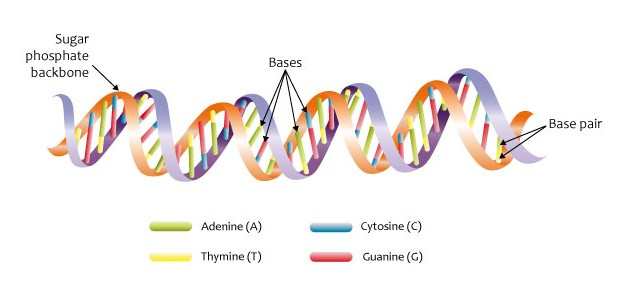
\includegraphics[width=\textwidth,natwidth=625,natheight=307]{dna.jpg}
   \caption[The structure of DNA]{The structure of DNA is based on the repeated pattern of a sugar and phosphate group, known as the sugar phosphate backbone, and the base pairing of the four bases, adenine (A), cytosine (C), guanine (G), and thymine (T). Image by NHS National Genetics and Genomics Education Centre licensed under the Creative Commons license.}
   \label{fig:dna}
\end{figure}

The definition of a gene has evolved with our increasing knowledge of genetics and biochemistry\cite{pmid17567988}. The idea of a gene dates back to Gregor Mendel when he demonstrated in his plant breeding experiments that discrete traits could be inherited from parents to offspring. While the mechanism of inheritance wasn't clear at that time, these heritable traits were termed a gene. The ``one gene, one polypeptide" hypothesis was the idea that each gene was responsible for producing a single enzyme/protein in a biochemical pathway; this was formed after observing that mutations in Neurospora genes would cause defects in steps of a metabolic pathways\cite{pmid16578042}. The relationship between DNA and proteins was demonstrated by the use of artificial ribonucleic acid (RNA) and bacterial cells\cite{pmid14471390}. RNA is synthesised by an RNA polymerase, using DNA as a template, in a process known as transcription. By using RNA artificially created to be entirely composed of uracils, Matthaei and colleagues produced a protein entirely composed of the amino acid phenylalanine. This experiment demonstrated that nucleic acids contained a code for amino acids. This code, known as the genetic code, was later cracked three years later\cite{pmid5330357} and defined how information is encoded in the genetic material. Nirenberg and colleauges worked out that three nucleotides defined a codon and is translated into one of the 20 standard amino acids. This flow of information from nucleic acid to protein was described as the ``Central Dogma"\cite{crick1958protein}.

\section{DNA to RNA}

The genome is a store of biological information that requires the coordinated activity of enzymes and proteins to bring it to life. This is achieved via transcription, which is a highly regulated mechanism that begins with RNA polymerase attaching to DNA and processes the template DNA strand into a single-stranded RNA molecule (Figure ~\ref{fig:transcription}). Transcription results in two main classes of RNA or transcripts: (1) Protein-coding transcripts, where the RNA known as messenger RNA (mRNA) can be further translated into a protein molecule and (2) Non-coding transcripts, where the RNA molecule is the functional product. There are three different types of RNA polymerases in eukaryotic cells: Pol I transcribes the genes that encode most of the ribosomal RNAs (rRNAs); Pol II transcribes the mRNAs; and Pol III transcribes the genes for small regulatory RNA molecules, such as transfer RNA (tRNA). RNA polymerase binds upstream to the DNA that will be transcribed at a region known as the promoter. Promoters can be classified by their distance to the transcription start site (TSS), which are the first nucleotides transcribed by RNA polymerase. The core promoter is the closest to the TSS and contains specific DNA sequences or elements that are necessary for transcription. The core promoter elements include the TATA box (usually located 25 to 35 bases upstream of the TSS), the initiator element (Inr), the downstream promoter element (DPE), the TFIIB recognition element (BRE) and the CpG island (CGI). The proximal promoter is the next closest (at $\sim~250$ bp) and usually contains primary regulatory elements; distal promoters are even further upstream and contain additional regulatory elements. Transcription with Pol I and Pol III are similar, but the promoter sequences and activator proteins differ.

\begin{figure}[h]
   \centering
   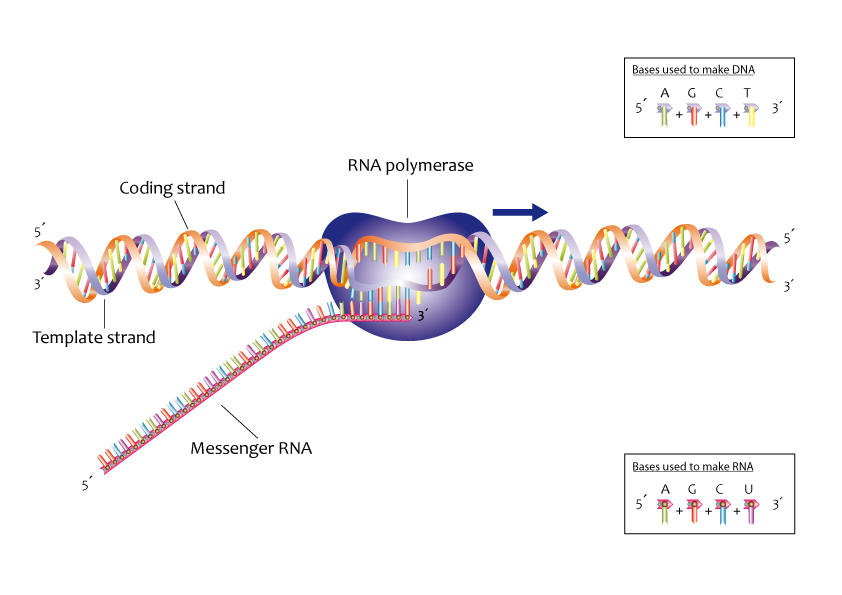
\includegraphics[width=\textwidth,natwidth=842,natheight=595]{transcription.jpg}
   \caption[DNA transcription]{The process of transcription begins with RNA polymerase, which reads the DNA sequence (the template strand) in the 5' to 3' direction and produces a complementary RNA strand called the messenger RNA (mRNA). The mRNA has the same sequence as the coding strand, except that thymines are replaced by uracils. Image by NHS National Genetics and Genomics Education Centre licensed under the Creative Commons license.}
   \label{fig:transcription}
\end{figure}

Transcription factors (TFs) are regulatory proteins that can activate or enhance the transcription of DNA by binding to specific DNA sequences at promoters (they are also known to negatively regulate transcription but this is less common). TFs contain one or more DNA-binding domains that allow it to bind to specific sequences. For example, the TATA binding protein (TBP), known as a general transcription factor (GTF), binds to the TATA box and is involved in DNA strand separation during transcription. Other GTFs include TFIIA, TFIIB, TFIID, TFIIE, TFIIF, and TFIIH, and are necessary for transcription to take place. Not all the GTFs bind to DNA but are part of the large transcription preinitiation complex (PIC) that interacts with RNA polymerase and helps position RNA polymerase over the TSS. As transcription takes place, the DNA double helix unwinds and RNA polymerase reads the template strand; the RNA sequence will have the same sequence as the coding strand.

The termination of transcription relies on terminator sequences that are found close to the ends of transcripts. For Pol I transcripts, transcription is stopped by a termination factor that unwinds the DNA-RNA hybrid formed during transcription. For Pol III transcripts, inverted repeats are transcribed and these sequences can form hairpin loops that pauses the RNA polymerase. For Pol II transcripts, a polyadenylation signal (AAUAAA) at the end of the sequence is necessary for termination\cite{pmid3479794}. The nascent RNA is cleaved at the polyadenylation site and a poly-adenine tail (poly(A)) is added; the poly(A) tail is important for the stability of the RNA, translation, and for nuclear export. In addition to this, a specialised nucleotide cap is added to the 5' end and this is the site recognised by the ribosomes in protein synthesis. The ribosome binds to the cap and reads along the 5' untranslated region (UTR) until it reaches an initiation codon. Removal of the cap is considered to the first step towards mRNA degradation. The capping procedure is thought to occur only in the nucleus, however a cytoplasmic form of a capping enzyme has been identified\cite{pmid22921400}. The default state of transcription in eukaryotes is that most genes are not constantly transcribed, unlike in prokaryotes. Structural properties of DNA make it inaccessible to the PIC; chromatin structure and nucleosome positioning are altered in order for the transcriptional machinery to access parts of the genome for transcription.

\section{DNA packaging}

Inside every somatic nucleated cell in the human body are 23 pairs of chromosomes; these chromosomes make up the human genome. A chromosome is a long DNA molecule that is condensed so that it may physically fit inside the nucleus (Figure ~\ref{fig:dna_condensed}). We can estimate the physical length the human genome by multiplying the number of base pairs contained on each chromosome by the length of a base pair. The haploid human genome contains around 3\e{9} base pairs of DNA; therefore there is a total of 6 billion base pairs of DNA per cell. Given that each base pair of DNA is about 0.34 nanometers long or 3.4\e{-10} meters\cite{pmid7354864}, each diploid cell contains 3.4\e{-10} * 3\e{9} * 2 or 2.04 meters of DNA. Given that the estimated number of cells in the human body is around 3.7\e{13} or 37 trillion\cite{pmid23829164}, a typical person contain around 74 trillion meters of DNA. Certain proteins, called histones, help compact the vast amounts of DNA inside of us (specifically, inside the eukaryotic nucleus). The histones are a family of small, positively charged proteins that provide the energy, in the form of electrostatic interactions, to fold negatively charged DNA (due to the phosphate groups in its phosphate-sugar backbone). The core histones are H2A, H2B, H3, and H4 and the resulting DNA-protein complex is called chromatin.

\begin{figure}[h]
   \centering
   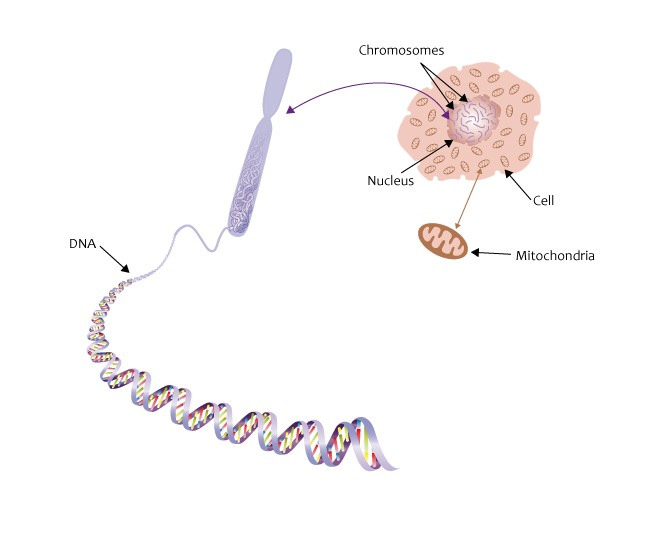
\includegraphics[width=\textwidth,natwidth=650,natheight=539]{dna_condensed.jpg}
   \caption[Condensation of DNA]{DNA is condensed into chromosomes by forming DNA-protein complexes known chromatin, which is further coiled into thicker fibers called 30nm fibers. The chromosomes reside inside the nucleus of a cell. Mitochondria also contain its own DNA. Image by NHS National Genetics and Genomics Education Centre licensed under the Creative Commons license.}
   \label{fig:dna_condensed}
\end{figure}

Chromatin possesses a fundamental repeating structure\cite{holde01111974}, known as nucleosomes and the packaging of DNA into nucleosomes shortens DNA about sevenfold. However despite this, chromatin is still too long to fit inside the nucleus, which is approximately 10 to 20 microns in diameter. Chromatin is further coiled into a thicker fiber, called the 30nm fiber, because it is roughly 30 nanometers in diameter. Processes such as transcription and replication require the two strands of DNA to come apart temporarily, thus allowing polymerases access to the DNA template. However, the presence of nucleosomes and the folding of chromatin into 30-nanometer fibers pose barriers to the enzymes that unwind and copy DNA. It is therefore important for cells to have means of opening up chromatin fibers and/or removing histones transiently to permit transcription and replication to proceed. Generally speaking, there are two major mechanisms by which chromatin is made more accessible:

\begin{enumerate}
   \item Histones can be enzymatically modified by the addition of acetyl, methyl, or phosphate groups.
   \item Histones can be displaced by chromatin remodelling complexes, thereby exposing underlying DNA sequences to polymerases and other enzymes.
\end{enumerate}

These two processes are reversible, so modified or remodelled chromatin can be returned to its compact state after transcription and/or replication are complete. The common nomenclature of histone modifications is by the name of the histone (e.g. H3), the single-letter amino acid abbreviation (e.g. K for lysine) and its position (e.g. 27), and the type of enzymatic modification (e.g. acetylation); put together this is represented as H3K27ac. Specific histone modifications are linked to different biological states; for example, acetylation removes the positive charge on the histones, decreasing the interaction between histones and DNA, leading to transcriptional activation. On the other hand, the tri-methylation of lysine 27 on histone H3, i.e., H3K27me3, is associated with the inhibition of transcription\cite{pmid21652639}. Given that distinct histone modifications can either activate or repress transcription, a ``histone code" has been proposed\cite{pmid11498575} and the profiling of the histone states will provide clues to the transcriptional state of a DNA region.

\section{DNA sequencing}

The process of DNA sequencing is the determination of the exact order of nucleotides within a DNA molecule. The first generation of DNA sequencing methods consisted of the electrophoretic methods (Sanger and Maxam-Gilbert sequencing), which were very labour intensive, requiring 4 separate reactions for the determination of each base. One of the first innovations was the use of different fluorophores with Sanger sequencing, which allowed the reactions to be pooled together during gel electrophoresis and eliminated the use of radioactive material. Automation of the DNA sequencing process was possible with the development of an apparatus that could detect the fluorescence emitted by the chain terminated fragments. This development was key towards the success of the Human Genome Project (HGP). For over 25 years since its inception, Sanger sequencing was the method of choice for DNA sequencing.

\subsection{Sanger and Maxam-Gilbert sequencing}

Sanger sequencing\cite{pmid271968} and Maxam-Gilbert sequencing\cite{pmid265521} were two methods of DNA sequencing developed in the 1970s requiring the use polyacrylamide gel electrophoresis, which allowed the resolution of DNA fragments at a 1 bp resolution, and allowed the determination of the DNA bases. The key feature of Sanger sequencing is the use of dideoxynucleotide triphosphates (ddNTPs) and a purified DNA polymerase enzyme to synthesise DNA. The structure of a normal nucleotide (dNTP), consists of a 3' hydroxyl (OH) group in the pentose sugar. The chain-terminating ddNTPs lack the OH group that is necessary for the formation of the phosphodiester bond between one nucleotide and the next during DNA strand elongation. If a ddNTP is incorporated into a growing DNA strand, the strand elongation is terminated. The idea is to set up a reaction with a mixture of dNTPs [deoxyadenosine triphosphate (dATP), deoxyguanosine triphosphate (dGTP), deoxycytidine triphosphate (dCTP), deoxythymidine triphosphate (dTTP)] and one particular ddNTP in a ratio of 300:1. Most of the times, the DNA will be elongated but once the ddNTP is incorporated the strand stops. This results in a number of DNA fragments of varying lengths and depending on the ddNTP used, the last base of the fragment corresponds to that base. This reaction is carried out for the other ddNTPs and all the fragments are separated using polyacrylamide gel electrophoresis. By reading the ladder, the DNA bases can be deduced. The Maxam-Gilbert sequencing method relies on the use of chemicals that can cleave specific bases. Dimethyl sulfate is used to cleave purine bases (A and G) and hydrazine is used to cleave pyrimidine bases (C and T). To distinguish the purines, an adenine-enhanced cleavage step is carried out, which cleaves adenines preferentially. To distinguish the pyrimidines, NaCl is used with hydrazine to suppress the reaction of thymines. As with Sanger sequencing, the DNA fragments are separated using polyacrylamide gel electrophoresis, and the DNA bases are deduced by reading the gel.

Sanger sequencing became the \textit{de facto} method for DNA sequencing due to its comparative ease and the use of fewer toxic materials than Maxam-Gilbert sequencing. A further improvement to Sanger sequencing replaced the need to radioactively label the DNA fragments by using chemically synthesised fluorescent oligonucleotide primers\cite{pmid3713851}. Four different fluorophores were used for each ddNTP reaction allowing all four reactions to be co-electrophoresed and the DNA sequence was deduced by reading the fluorescence colours. The development of a fluorescence detection apparatus linked to a computer that processed the data created the world's first partially automated DNA sequencer\cite{pmid3713851}.

\subsection{Next-generation sequencing}

The next wave of DNA sequencing methods, the so-called next-generation (next-gen) or second generation sequencing, started with various strategies that rely on a combination template preparation, sequencing, and imaging that allowed thousands to billions of sequencing reactions to be performed simultaneously\cite{pmid19997069}. Next-gen sequencing relies on the clonal amplification of templates and use \textit{in vitro} cloning rather than bacterial cloning; the two most common methods are emulsion PCR (emPCR)\cite{pmid12857956} and solid-phase amplification\cite{pmid16473845}. With emPCR individual DNA molecules are isolated with primer-coated beads in water-in-oil microreactors and clonal amplification leads to thousands of copies of the DNA molecule in an emulsion. 454 pyrosequencing and SOLiD sequencing use emPCR, where the amplification product is deposited into individual wells for sequencing. Solid-phase amplification relies on a lawn of high-density primers that are covalently attached on a slide surface (also known as a flow cell) and bind to DNA molecules ligated with sequencing adaptors. The two methods allow each DNA template to be spatially separated, allowing massively parallel sequencing to take place.

Sequencing can take place via the use of DNA polymerase, which is commonly known as sequencing-by-synthesis, and via the use of DNA ligase, known as sequencing-by-ligation (SBL). SBS can be further classified into cyclic reversible termination (CRT), single-nucleotide addition (SNA) and real-time sequencing\cite{pmid19997069}. CRT uses reversible terminators and initial developments used the same dideoxynucleotides used as chain terminators in Sanger sequencing. The concept of CRT is that a DNA polymerase incorporates one fluorescently modified nucleotide, which has a reversible terminator that terminates DNA synthesis. Unincorporated nucleotides are washed away and fluorescence imaging takes place to determine the identity of the incorporated nucleotide. The last step removes or cleaves the reversible terminator and the fluorescent dye and the cycle is repeated. The CRT method is used in Solexa/Illumina and Helicos sequencing. SBL relies on DNA ligase and either one-base-encoded or two-base-encoded probes that are fluorescently labelled. The probes hybridise to its complementary sequence on the primed template and DNA ligase is added to join the probe to the primer. Non-ligated probes are washed away followed by fluorescence imaging and cleavage of the fluorescent dye and the cycle is repeated. The SBL method is used in SOLiD sequencing.

The third generation of sequencing loosely refers to single-molecule sequencing technologies, which have the capacity for longer read lengths at potentially cheaper costs\cite{pmid20858600}. One of the main advantages of single-molecule sequencing is that PCR is not required, therefore amplification biases and PCR mutations are eliminated. Furthermore, quantitative applications of sequencing such as RNA sequencing (RNA-Seq) are much more representative of the true abundance of RNA molecules. The HeliScope sequencer was the first commercially available single-molecule sequencer, which was based on the work of Stephen Quake and colleagues\cite{pmid12651960}. HeliScope sequencing utilises billions of primed single-molecule templates are covalently attached to the solid support and uses CRT but with slight differences from Solexa/Illumina sequencing. HeliScope uses Helicos Virtual Terminators, which differ from the reversible terminators used in Solexa/Illumina sequencing and dye labelled nucleotides are added individually in the predetermined order of C, T, A, and G, which is followed by fluorescence imaging.

With the advent of next-gen sequencing we have the capacity to sequence an entire human genome in a matter of days. Developments in next-gen sequencing are aiming towards longer read lengths with higher output (Figure ~\ref{fig:dev_next_gen}) and we have just recently arrived in the \$1,000 genome era, whereby we can sequence the entire genome of an individual for around \$1,000 US dollars (USD). In contrast, the Human Genome Project (HGP), which gave us the first glimpse of the human genome\cite{lander2001initial} costed approximately 2.7 billion fiscal year 1991 US dollars\cite{nhgri2010cost}. Next-gen sequencing is also not just limited to genome sequencing; reverse transcriptase\cite{pmid4316300, pmid4316301} allow for the synthesis of complementary DNA (cDNA) from RNA and therefore the entire collection of RNA, known as the transcriptome, can be sequenced. Other applications of next-gen sequencing has allowed us to capture in a genome-wide manner DNA-protein interactions, DNA methylation patterns, and histone modifications\cite{applicationsofsequencing}.

\begin{figure}[h]
   \centering
   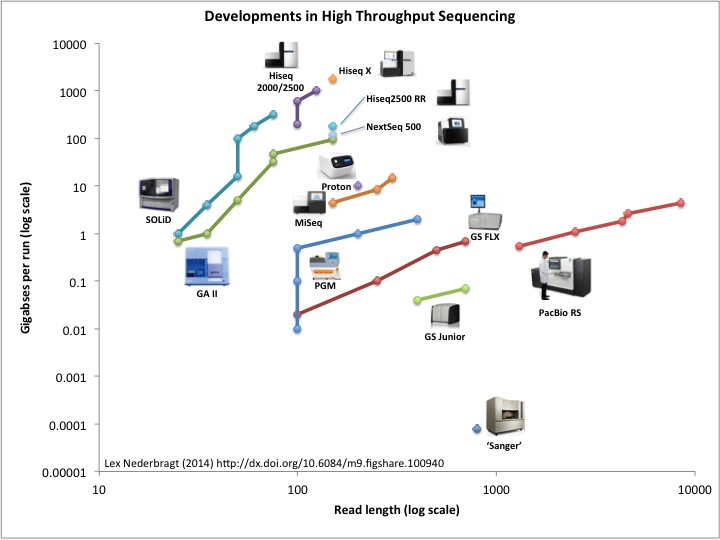
\includegraphics[width=\textwidth,natwidth=720,natheight=540]{developments-in-next-generation-sequencing.jpg}
   \caption[Developments in next generation sequencing]{Log read length versus log gigabases per run for various next generation sequences\cite{Nederbragt2012}.}
   \label{fig:dev_next_gen}
\end{figure}

\section{Applications of sequencing}

There is a large number of *Seq protocols\cite{pachter2014seq}, which is set to increase with the decrease in sequencing costs and the development of innovations in molecular biology.

The age of high throughput sequencing and the application of this technology to studying the transcriptome (also epigenome and interactome).

One of the first technologies that allowed the simultaneous profiling of thousands of transcripts was microarrays and with the development of whole-genome arrays, the whole repertoire of known transcripts could be assayed. However, with the advent of high-throughput sequencers, RNA sequencing (RNA-Seq) became an attractive alternative to microarrays. RNA-Seq is an application of high-throughput sequencing that is used to study RNA expression levels in a discovery-based manner, since it does not rely on any \textit{a priori} knowledge of transcripts. RNA-Seq gives digital gene expression (DGE) profiles, which provides a large dynamic range of expression values and is much more quantitive than microarrays. Furthermore, RNA-Seq does not suffer from cross-hybridisation issues when profiling transcripts from repetitive regions of the genome.

RNA-Seq is relatively new compared to microarray technology, which has been around since 1995, but is gaining more widespread use due to the rapid drop in sequencing costs. As such RNA-Seq protocols are continually being developed and improved upon to avoid any biases. Methods used for storing, analysing, and visualising RNA-Seq data are also being heavily researched upon. In the near future, RNA-Seq may be used as routinely as microarrays for performing transcriptome profiling.

Non-coding RNAs, which include small and long non-coding RNAs, contribute to a significant portion of the transcriptome in mammalian genomes. However, the functional significance of this wide-spread occurrence of ncRNAs for organismal development and differentiation is unclear. While coding transcripts serve mainly as templates for protein synthesis, the functions of some well known non-coding transcripts are diverse. Furthermore, the major portion of many mammalian genomes are occupied by DNA sequences that are repetitive.

Technologies for the interrogation of nucleic acids have made it possible to investigate different biological questions.

\subsection{Transcriptomics}

The transcriptome is the collection of RNA molecules derived from the genome at a particular time and location. The diversity of cells is determined by the expression patterns of genes and transcription factors (TFs).

\subsection{Transcription regulation}

Control of the frequency and rate of transcription and by the stability of the transcripts and translational efficiency for protein-coding transcripts.

Methylation of specific bases in the DNA.

\subsection{Characterising the transcriptome}

 The transcriptome is the total output of RNA in a cell (or cells in a tissue) at a certain period of time. The characterisation of the transcriptome involves assessing the amount of output from all transcripts that are expressed. It should be noted that measurements of expression depend on not only the transcriptional activity of the transcript but also the stability since these methods capture the total RNA expression at a specific time.

The number of cycles needed for formation of a detectable amount of product, known as the cycle threshold ($C_{t}$) value, is related to the initial amount of template and higher amounts of initial template will result in lower $C_{t}$ values. If you are comparing the levels of mRNA from different samples, the overall starting amount of RNA must be the same. The best way of standardising the template is to carry out a parallel RT-PCR using another gene that is known to be constitutively expressed such as beta-actin or GAPDH.

Microarrays\cite{pmid7569999}

Studies on the yeast transcriptome using DNA microarrays showed that although mRNAs are being degraded and re-synthesised all the time, the composition of the yeast transcriptome undergoes very little change if the environment remains constant\cite{pmid9381177}
However on switching from aerobic to anaerobic respiration, the levels of over 700 mRNAs increase by a factor of two or higher, and another 1,000 mRNAs decline to less than half their original amount
Studying the transcriptome of acute lymphoblastic leukemia cells with respect to acute myeloid leukemia cells revealed differences that made it possible to distinguish the two types of leukemia

\begin{itemize}
   \item Pervasive transcription describes the observation that a large percentage of DNA in mammalian genomes is transcribed.
   \item Tiling arrays and full length cDNA sequencing suggested that most of the genome is transcribed
   \item The ENCODE pilot project provided multiple lines of evidence that most of the mammalian genome is associated with at least one primary transcript, i.e., pervasive transcription of the genome
   \item Are the majority of detected low-level transcription due to technical artifacts and/or background biological noise?
   \item Protocols that capture only poly-A transcripts as opposed to poly-A minus and cytoplasmic versus nuclear enrichment libraries
   \item Sequencing depth and sampling of RNA molecules; absolute transcript quantification will help (such as using unique molecule identifiers and non-PCR based methods)
   \item Functional transcriptomics in the post-ENCODE era, specifically what is the criteria for functionality
   \item Collection of mouse full length cDNAs by the FANTOM consortium revealed many transcripts of unknown function (TUFs)
   \item 38.6\% of the FANTOM3 mouse full-length cDNAs have very low coding potential (CPAT coding probability of less than 0.2) (Figure ~\ref{fig:fantom3_coding_prob})
   \item The technologies that allowed full length cDNA sequencing
   \item PacBio sequencing has read lengths greater than 10kb and can be used for full length cDNA sequencing

\end{itemize}

\begin{figure}[h]
   \centering
   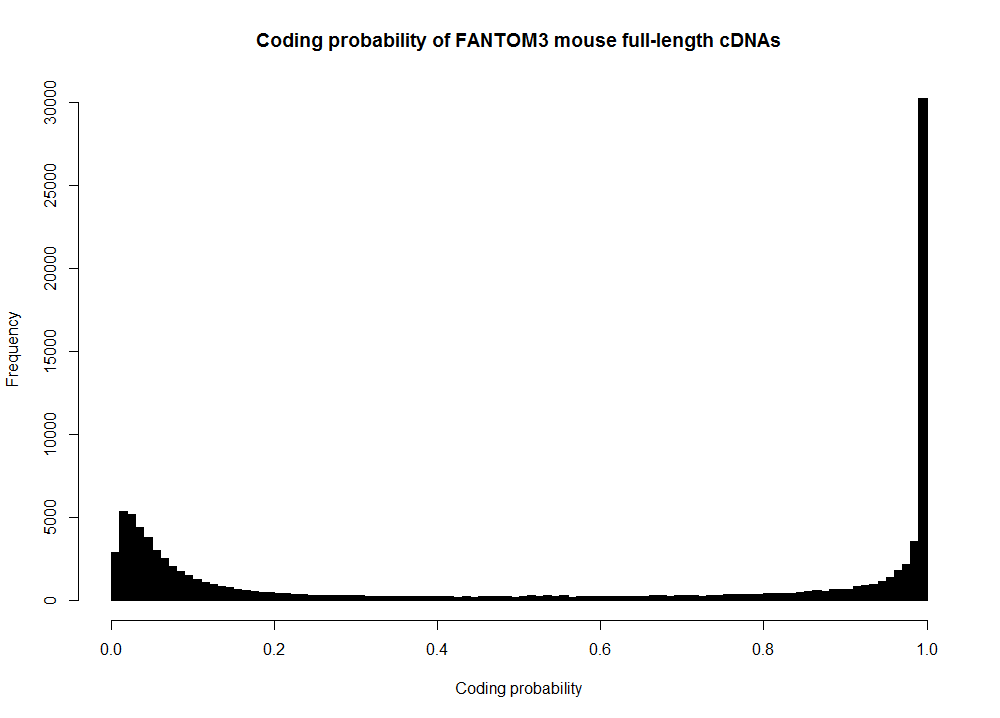
\includegraphics[width=\textwidth,natwidth=1000,natheight=718]{fantom3_coding_probability.png}
   \caption[Coding probability of FANTOM3 mouse cDNAs]{Distribution of coding probabilities of FANTOM3 mouse full-length cDNAs as predicted by CPAT\cite{tang2014fantom3codingprob}.}
   \label{fig:fantom3_coding_prob}
\end{figure}

\subsection{Cap Analysis Gene Expression}

Cap Analysis Gene Expression (CAGE) was conceived as a method to detect all known transcription factors and active promoters for understanding the interplay between the two\cite{carninci2010capanalysis}. At that time sequencing was still relatively expensive and thus came the idea of cutting and concatenating 5' ends of full-length cDNAs, followed by sequencing. The use of CAGE in the FANTOM3 project unveiled the transcriptional landscape of the mammalian genome\cite{pmid16141072}, which identified many novel mRNAs and non-coding RNAs. Insight into the promoter architecture was also revealed by CAGE, where two major classes were discovered: conserved TATA box-enriched promoters and CpG-rich promoters\cite{pmid16645617}. FANTOM4\cite{pmid19377474}. FANTOM5\cite{pmid24670764}.

Regulatory regions will control the rate of transcription for a gene. Experimental validation include cloning fragments of DNA around and upstream from the transcription start site of a gene and testing for promoter activity by using a vector that carries a promoterless reporter gene. This approach can test whether a DNA fragment has promoter activity or not but the specific sequence that confers the promoter activity is unknown as well as the transcription factors that interact with the DNA fragment. Using mutagenesis it is possible to test how different mutations affect the promoter activity.

One such technology for capturing TSSs is called Cap Analysis Gene Expression (CAGE), which essentially captures RNA that have a cap structure (specifically biotinylation of diol groups of RNA\cite{pmid8938445}) and sequences them. The cap is right at the start of a precursor transcript, thus this position represents the TSS. The output of CAGE is a set of short tags that correspond to the capped RNAs, with the number of tags reflecting the abundance of the RNAs.

Cap Analysis Gene Expression (CAGE) for genome-wide identification of transcription start sites

\subsection{Non-coding RNAs}

Diverse class of non-coding RNAs, broadly broken down into long and short non-coding RNA

Classical non-coding RNA found in both prokaryotes and eukaryotes are ribosomal RNAs and transfer RNAs, which are both involved in protein synthesis

Micro-RNAs (miRNAs) were first first observed in 1993 in Caenorhabditis elegans\cite{pmid8252621} as a small double-stranded RNA that were bound to the 3' untranslated region (UTR) of an mRNA. The binding of the miRNA inhibited the translation of the mRNA and is one of the mechanisms by which miRNAs post-transcriptionally regulate gene expression. The biogenesis of miRNAs begins with the cleavage by an enzyme called Dicer\cite{pmid11201747}, which is part of the RNase III family. miRNAs inhibit translation by recruiting a ribonucleoprotein complex called RNA-induced silencing complex (RISC). Short-interfering RNAs are also cleaved by Dicer and can also bind to mRNA but require complete complementarity. MiRNAs are products of dsRNAs encoded in genes in our genome and do not require full complementarity to bind to a target mRNA thus one miRNA may regulate several genes.

A single-stranded nucleic acid molecule will tend to fold up on itself to form localised double-stranded regions, producing structures called hairpins or stem-loop structures. This is due to the hydrophobic nature of the bases, which means that the bases are unstable when exposed to an aqueous environment. Pairing of the bases enables them to be removed from interaction with the surrounding water and stabilising the DNA helix.

Assembly of non-coding RNAs with proteins as ribonucleoprotein (RNP) structures
Interaction of non-coding RNAs with chromatin

\section{The repetitive genome}

Since the release of the draft human genome sequence\cite{venter2001sequence, lander2001initial}, it was established that only a small fraction of the genome is made up of protein-coding sequences and the majority of the genome was made up with repetitive elements. As the human genome contains the entire instruction set that is necessary for the development of a human, the decoding of the genome was thought to provide answers to many outstanding biological questions. However, there are several paradoxes that are still currently unresolved:

\begin{enumerate}
   \item K-value paradox: complexity does not correlate with the number of chromosomes
   \item C-value paradox: complexity does not correlate with genome size
   \item N-value paradox: complexity does not correlate with the number of protein coding genes
\end{enumerate}

If we measure organismal complexity in terms of mental cognition, we observe that complexity is not correlated to the number of chromosomes, the size of genomes, and the number of protein coding genes. Humans have 46 chromosomes and some species of butterflies have over hundreds of chromosomes, such as \textit{Polyommatus atlantica}. In terms of genome size, the species \textit{Polychaos dubium}, a freshwater amoeboid, has one of the largest genomes known with around 670 gb of DNA sequence; humans on the other hand have a genome size of roughly 3 gb. And lastly humans have roughly the same number of protein-coding genes as \textit{Caenorhabditis elegans}, roughly 20,000 versus 21,000, respectively. However, the \textit{C. elegans} genome is about 100 mb\cite{celegans1998sequencing}, which is approximately 30 times smaller than the human genome, despite having a similar number of genes. One of the discrepancies between genome sizes despite having a similar number of genes is due to repetitive elements, which makes up roughly 50\% of the human genome. Among 66 vertebrate genomes, the percentage coverage of repetitive elements in the human genome is quite high (Figure ~\ref{fig:repeat_coverage_vertebrate_genome}).

\begin{figure}[h]
   \centering
   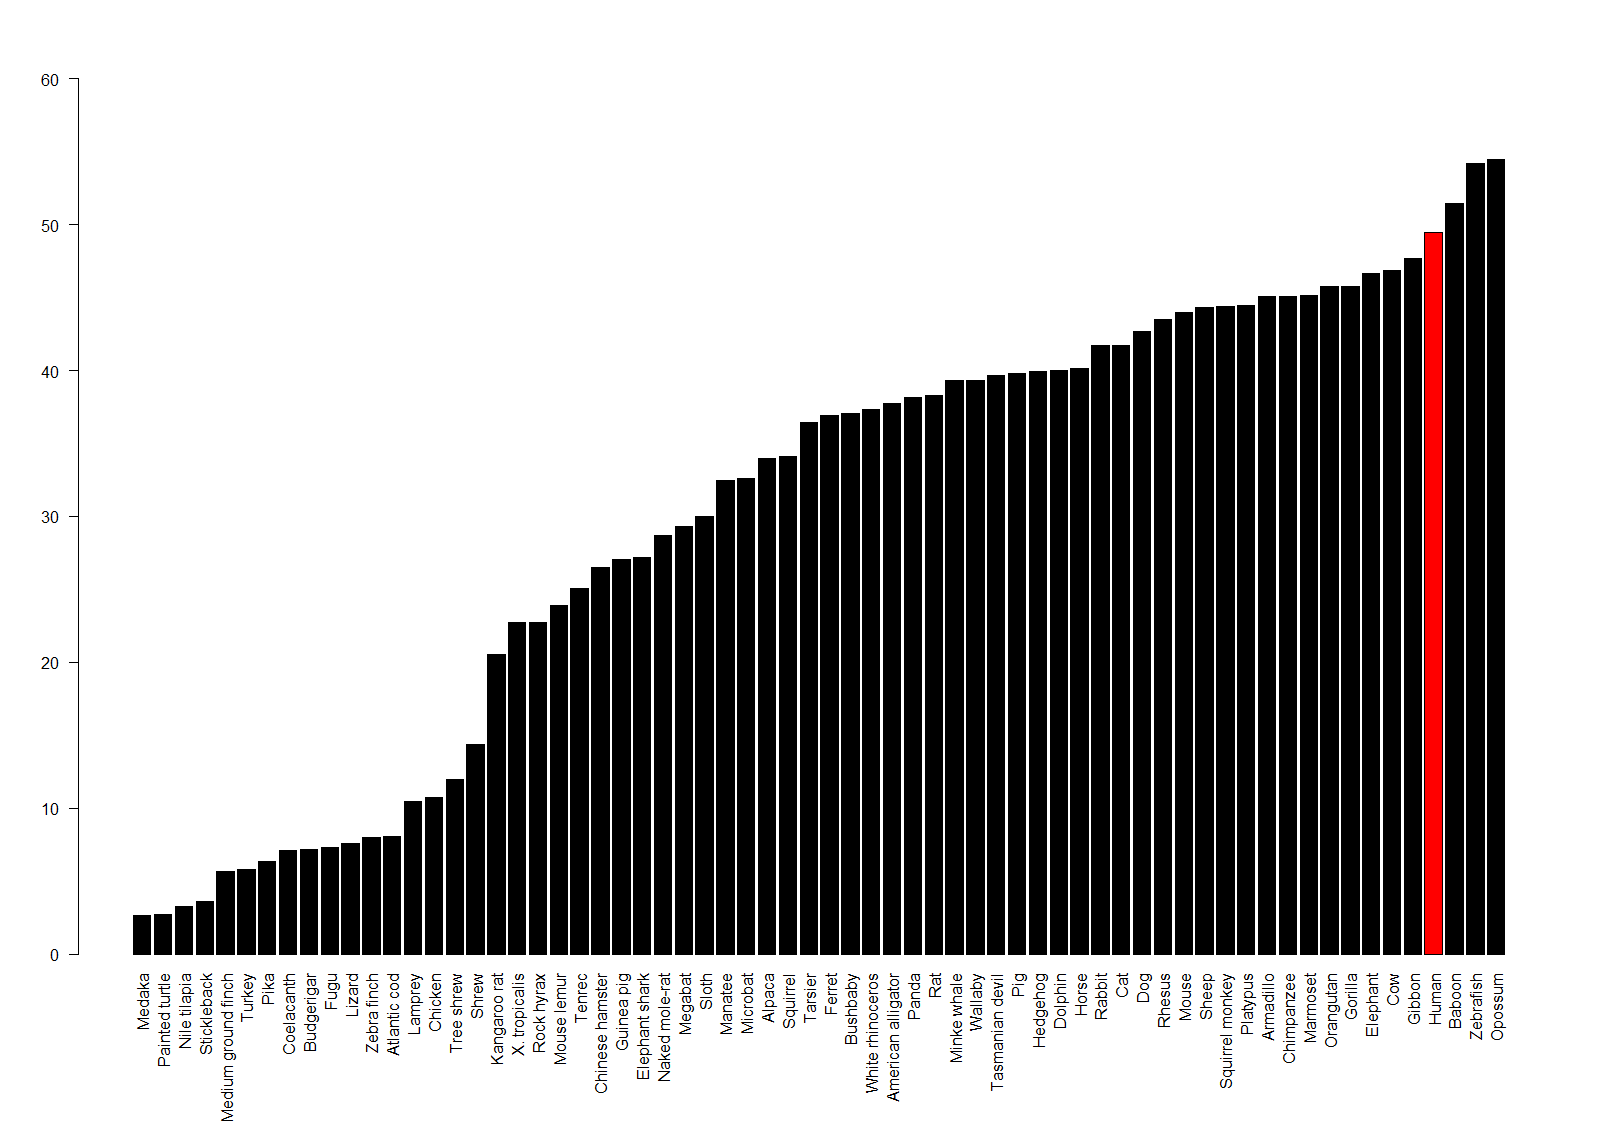
\includegraphics[width=\textwidth,natwidth=1600,natheight=1148]{repeat_coverage_vertebrate_genome.png}
   \caption[Coverage of repetitive elements in vertebrate genomes]{The total coverage of repetitive element in 66 vertebrate genomes as annotated by RepeatMasker in the respective genomes\cite{tang2014repcoverage}.}
   \label{fig:repeat_coverage_vertebrate_genome}
\end{figure}

However, the larger vertebrate genomes do not always contain the highest percentage of repetitive elements (Figure ~\ref{fig:genome_size}). At least in humans, transposons make up the majority of the repetitive elements that make up the human genome. In particular class I transposons (retrotransposons), which are able to transcribed and inserted into the genome, make up a large portion of the human genome. W.Ford Doolittle and Carmen Sapienza wrote in 1980\cite{doolittle1980selfish}: ``When a given DNA, or class of DNAs, of unproven phenotypic function can be shown to have evolved a strategy (such as transposition) which ensures its genomic survival, then no other explanation for its existence is necessary" and Leslie Orgel and Francis Crick, wrote that junk DNA has little specificity and conveys little or no selective advantage to the organism\cite{orgel1980selfish}.

The origin of the term ``junk DNA" is usually attributed to Susumu Ohno, who used it to describe pseudogenes, which are gene copies that have no known biological function. In its modern day usage, ``junk DNA" is used to describe DNA sequence that goes not play a functional role in an organism. Dr. Ohno estimated that there would be an upper limit to the number of functional loci in mammalian genomes based on mutational load and a fixed mutation rate. He predicted that mammalian genomes could not have more than 30,000 loci under selection as this would guarantee a progressive decline in fitness, leading to extinction.

\begin{figure}[h]
   \centering
   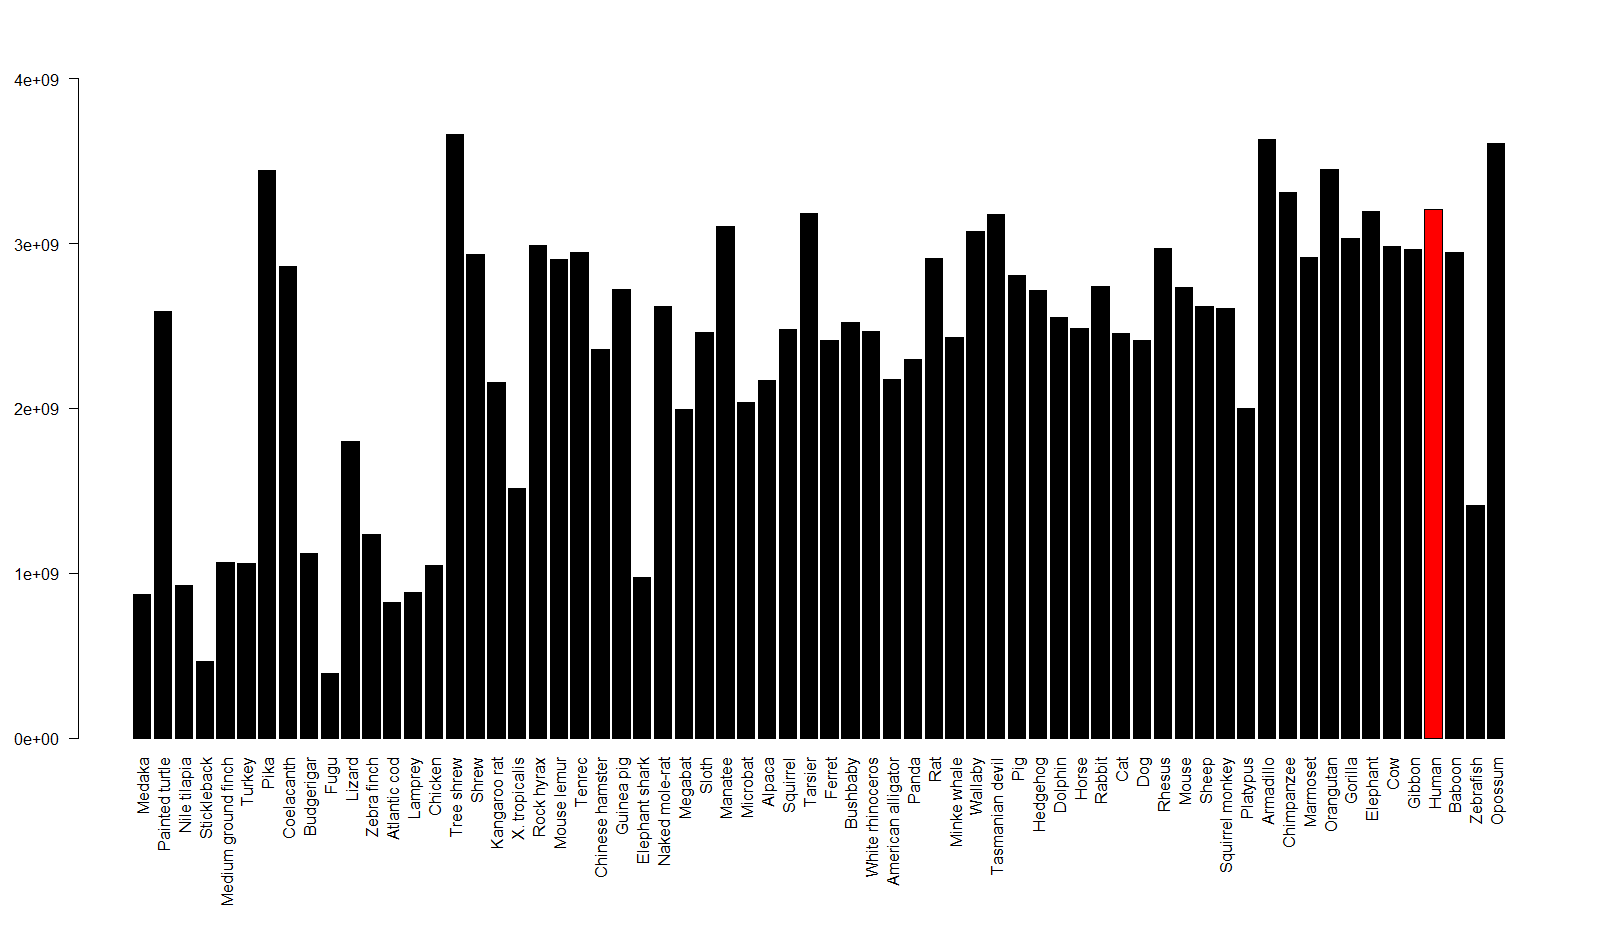
\includegraphics[width=\textwidth,natwidth=1600,natheight=932]{genome_size.png}
   \caption[Vertebrate genomes sizes]{The genome sizes of 66 vertebrate genomes, sorted from the lowest to highest percent of repetitive element coverage\cite{tang2014gensize}.}
   \label{fig:genome_size}
\end{figure}

\begin{figure}[h]
   \centering
   \includegraphics[width=9cm, angle=270]{barplot_repeat_family.eps}
   \caption[Tally of repetitive element families in the hg19 genome]{The number of repetitive element families determined by RepeatMasker in the hg19 genome.}
   \label{fig:repeat_family}
\end{figure}

\begin{itemize}
   \item Repeat-associated binding sites (RABS) are over-represented in proximity of regulated genes and that the binding motifs within these repeats have undergone evolutionary selection
   \item Indeed, studies conducted both at the gene and genome levels have uncovered TE insertions that seem to have been co-opted - or exapted - by providing transcription factor binding sites (TFBSs) that serve as promoters and enhancers, leading to the hypothesis that TE exaptation is a major factor in the evolution of gene regulation.
   \item The transcription of repetitive elements, especially transposable elements, in specific tissues
   \item Repetitive elements are usually highly methylated, however differentiation methylation patterns of repetitive elements was observed in specific tissues
   \item Functions of some GWAS candidates in intergenic regions (such as http://www.nature.com/nature/journal/v507/n7492/full/nature13138.html)
   \item The regulated retrotransposon transcriptome of mammalian cells\cite{pmid19377475}
\end{itemize}


\section{Stem cells}

The existence of stem cells was discovered in 1961 and the stem cell theory was published in 1963\cite{pmid13970094}. In this work, Canadians researchers James Till and Ernest McCulloch proved that stem cells were present in bone marrow. They exposed mice to high doses of radiation that killed off the mouse's blood and immune forming system and then injected bone marrow cells into some of the mice. The mice that didn't receive the transplants died and the mice that received the transplants survived because the bone marrow cells rebuilt their blood and immune forming systems. The bone marrow cells were able to reproduce themselves as well as generating different cell types. Human bone marrow transplants are still routinely used nowadays to treat leukaemia and other kinds of blood disorders.

Stem cells have two key characteristics that differ from other cells: they can reproduce themselves for long periods of time, known as self-renewal, and they can differentiate or specialise into specific cell types under certain conditions. What Till and McCulloch discovered were actually adult or tissue stem cells (ASCs), which are multipotent; this means that they have limited differentiation ability and are only able to generate specific types of differentiated cells. For example, haematopoietic stem cells, which are a type of adult stem cells that reside in the medulla of the bone (bone marrow), are only able to give rise to different mature blood cell types and tissues. In 1981, researchers were able to derived embryonic stem cells (ESCs) from mouse embryos (specifically the inner cell mass of blastocysts) and grow them on Petri dishes\cite{pmid7242681, pmid6950406}. In normal development, the inner cell mass begins growing into all the different cell types of the fully developed body and as such ESCs are able to differentiate into all the cell types that make up the body and they are pluripotent. Cells with the highest potency or with the most differentiation potential, are known as totipotent cells and are able to form all the cell types in a body, including the placental cells. Embryonic cells within the first couple of cell divisions after fertilisation are the only cells that are totipotent.

In 2006, a new methodology was invented by Takahashi and Yamanaka to generate another type of stem cell, called induced pluripotent stem cells (iPSCs)\cite{pmid16904174}. In their work, they discovered a way to generate pluripotent stem cells from somatic cells, which have no differentiation potential. Since their discovery, many researchers wondered about the development potential of iPSCs and in 2009 a Chinese group were successful in creating a live mice from iPSCs that were able to produce offspring\cite{pmid19672241}. In one of the first studies to show the clinical application of human iPSCs to human disease, a team derived iPSCs from fibroblasts of patients suffering from alpha 1 antitrypsin deficiency, corrected the disease causing mutation, and used the corrected stem cells to produce liver cells that were transplanted into the liver via intrasplenic injection\cite{pmid21993621}. Since the cells are genetically identical to the patient, there is no worry about rejection or immune problems, and is one reason why iPSCs are an attractive option for regenerative medicine.

\section{The role of bioinformatics in genomics}

Modern day high-throughput sequencers generate large amounts of data; for example in the blood transcriptome project (Chapter 7), one lane of sequencing on the HiSeq2000 produced 74.5 million reads (using 15 gigabytes of storage space when uncompressed). To deal with data at this scale, informatics tools for storing, managing, and analysis such data sets are absolutely necessary. Bioinformatics can be thought of as informatics for biological data, though historically it was defined as ``the study of informatic processes in biotic systems"\cite{pmid21483479}. The HGP was one of the first large scale international research efforts and bioinformatics was crucial towards the successful completion of the HGP\cite{stein1996perl}. An important principle established during the HGP, called the ``Bermuda Principles", was set by an international assortment of genome-research leaders towards the rapid and public sharing of human genome information. These set of commitments left a lasting legacy in large genomic science projects such as The International HapMap Project, ENCODE and modENCODE, and The Cancer Genome Atlas where data was made freely available prior to publication\cite{contreras2011bermuda}. The public availability of data from these projects have resulted in major advances in genomics and bioinformatics.

The FASTQ format was formally defined in 2010\cite{pmid20015970} and has become the \textit{de facto} format for storing raw sequencing output. FASTQ is similar to the FASTA format with the addition of storing quality scores for each nucleotide. The format is simplistic, which may be the reason for its popularity before being formalised. The establishment of a standard format is important as developers can produce programs, such as sequence aligners, that can process output from different sequencing machines. Another standard file format for storing sequence alignments is the Sequence Alignment/Map (SAM) format\cite{pmid19505943}.

The reads generated from the second generation of sequencers were much shorter and much more numerous than traditional Sanger sequencing reads. The Illumina GAII can produce up to 100 million reads of 50 bp in a single run. Traditional sequence alignment tools using the Needleman–Wunsch algorithm or Smith–Waterman algorithm were simply too slow and new developments were necessary. The popular short-read alignment tool, BWA\cite{pmid19451168}, implements the Burrows–Wheeler transform to deal with the vast number of short reads.

Comparing genomic features using BEDTools\cite{pmid20110278}.

Expression data sets are commonly stored as matices; for example if we let $A$ be an $m \times n$ matrix, where $a_{ij}$ are elements of $A$, the $i^{th}$ row would represent the transcriptional response of the $i^{th}$ gene and the $j^{th}$ column would represent the expression profile of the $j^{th}$ assay:

\begin{align*}
   A = \begin{bmatrix} a_{11} & \cdots & a_{1j} & \cdots & a_{1n} \\
   . && . && . \\
   a_{i1} & \cdots & a_{ij} & \cdots & a_{in} \\
   . && . && . \\
   a_{m1} & \cdots & a_{mj} & \cdots & a_{mn} \end{bmatrix}
\end{align*}

A differential expression analysis can be easily performed on an expression matrix, such as by using the edgeR package\cite{pmid19910308} from Bioconductor\cite{pmid15461798}. Multidimensional scaling methods, such as Singular Vector Decomposition (SVD), can also be applied on the matrix to find underlying patterns in the data. A very popular visualisation method of expression data is the use of heatmaps that reflect the relative expression strength of each element in the matrix ($a_{mn}$), which is commonly used in tandem with hierarchical clustering. Co-expression matrices can be further derived from the expression matrix to find transcripts with a similar transcriptional response or assays with similar expression profiles. Networks or graphs can be built from such co-expression matrices for visual purposes or for analysing the structure of co-expression patterns.

